\documentclass {article}
\usepackage{graphicx}
\usepackage{amsmath}



\begin{document}


\section{Meta Theory}


Who, What, Where, When, Why, How?
\\[0.15in]
what?    A new theory of  gravity
\\
why?   100 years quantumgravity = GR + QM . Other proposals
\\[1in]

Moving Goal Posts
\\

MVP
\\

What is a theory?
\\[1in]

Hypothesis vs. Postulate vs. Assumptions? (Main Hypothesis with mathematical framework postulates?)
\\[1in]



What does a theory of gravitation need?
\\[2in]

What would be nice to have? 
\begin{itemize}
	\item Simplicity : Occam's razor
	\item A wow!
\end{itemize}

\vspace{10pt}





\newpage


\section{Maxwell Equations}
\subsection{From Electromagnetism to Gravity-magnetism}

We assume that gravity is correctly described by Maxwell's Equations:

$$\nabla \times \vec B  - \partial_t \vec E  = -4 \pi G \vec J ~~~~~~~~ \nabla \times \vec E + \partial_t \vec B = 0    ~~~~~~~~~~~ (1)$$

$$\nabla \cdot \vec E = -4 \pi G \rho ~~~~~~~~~~ \nabla \cdot \vec B = 0   ~~~~~~~~~~~ (2)$$

and, for completeness, the conservation of mass-charge:

$$\nabla \cdot \vec J + \partial_t \rho = 0 ~~~~~~~~~~~ (3)$$

Where we are in units where c = 1. The constant G differs in different systems of units. In SI units, it is equal to $6.674 \times 10^{-11} \frac {N \cdot m^2}{kg^2}$ 

\newpage 
\subsection{Solenoidal and Irrotational Vectors}
While this step is not strictly necessary, and all of the results in the rest of the paper can still be derived, it actually tends to make the math a little cleaner to split the Maxwell equations into their Irrotational and Solenoidal forms.

A vector $\vec V$ can be split into a solenoidal vector $\vec V_S$ and an irrotational vector $\vec V_I$:

$$\vec V = \vec V_I + \vec V_S $$

where

$$\nabla \cdot \vec V_S = 0 ~~~~~ \nabla \times \vec V_I = 0 $$

Using this notation we can rewrite the Maxwell equations into irrotational equations:

$$\nabla \cdot \vec E_I = -4 \pi G  \rho$$

$$\nabla \cdot \vec J_I + \partial_t \rho = 0 $$

$$ \partial_t \vec E_I = 4 \pi G \vec J_I $$

And solenoidal equations:

$$\nabla \times \vec E_S + \partial_t \vec B_S = 0 $$

$$\nabla \times \vec B_S - \partial_t \vec E_S =  - 4 \pi G \vec J_S$$

The thing we really want to say, and I'm not sure if this is an assumption or is just totally obvious, is that, at least when we are in the rest frame of the mass (which is the frame of reference that we will be in for the rest of this paper), these equations de-couple. We have one set of equations that describe the forces due to the mass and another set of equations that describe radiation. We can make this explicit by defining a new current:

$$\vec {J_S'} = - G \vec {J_S}$$

which changes the inhomogenous Solenoidal equation into:

$$\nabla \times \vec B_S - \partial_t \vec E_S =  4 \pi \vec {J_S'} $$

but affects none of the other equations at all!

Because this form of the equations is the same as that presented in books on radiation. I will get rid of the prime on the Solenoidal current, and use the following equations as the solenoidal (radiation) Maxwell equations:

$$\nabla \times \vec B_S - \partial_t \vec E_S =  4 \pi \vec J_S$$

$$\nabla \times \vec E_S + \partial_t \vec B_S = 0 $$
\newpage

\section{Solutions to the Maxwell Equations}
\subsection{Spherical Vectors}
Following Berrara (http://iopscience.iop.org/article/10.1088/0143-0807/6/4/014/meta) we assume that any vector field, $\vec V$, and any scalar, $g$, can be expanded as follows:

$$\vec V (\vec x) = \sum_{l=0}^{\infty} \sum_{m=-l}^{l} \left[a_{lm}(r) \vec Y_{lm}(\theta, \phi) +b_{lm}(r) \left( \hat r \times \vec X_{lm} (\theta, \phi) \right) +c_{lm}(r) \vec X_{lm} (\theta, \phi) \right] $$

$$g(\vec x) = \sum_{l=0}^{\infty} \sum_{m=-l}^{l} g_{lm}(r) Y_{lm}(\theta, \phi)$$

where $Y_{lm}$ are the usual spherical harmonics (see Jackson 3.53), $\vec Y_{lm}$ is simply $\hat r Y_{lm}$  and $\vec X_{lm}$ is defined as,

$$\vec X_{lm}(\theta, \phi) = \frac {-i}{\sqrt{l(l+1)}} \vec r \times \left( \nabla Y_{lm}(\theta, \phi) \right) $$

The three vector spherical harmonics $(\vec Y_{lm}, \vec X_{lm}, \hat r \times \vec X_{lm} )$ obey a few relations compiled below for ease of reference:

$$\nabla  \cdot \left( f(r) \left( \hat r \times \vec X_{lm} \right) \right) = - i \sqrt {l(l+1)} \frac {f(r)} {r} Y_{lm}$$

$$\nabla \cdot \left( f(r) \vec X_{lm} \right) = 0 $$

$$ \nabla \cdot \left( f(r) \vec Y_{lm} \right) = \frac {1}{r^2} \frac d {dr} \left(r^2 f(r) \right) Y_{lm}$$

$$\nabla \times \left( f(r) \left( \hat r \times \vec X_{lm} \right) \right) = \frac {-1} {r} \frac d {dr} \left( r f(r) \right) \vec X_{lm}$$

$$\nabla \times \left( f(r) \vec X_{lm} \right) = \frac {i \sqrt{l(l+1)} } {r} f(r) \vec Y_{lm} + \frac 1 r \frac d {dr} \left( r f(r) \right) \left( \hat r \times \vec X_{lm} \right)$$

$$\nabla \times \left( f(r) \vec Y_{lm} \right) = \frac {- f(r)} r i \sqrt {l (l+1)} \vec X_{lm}$$

$$ \vec X_{lm} \cdot ( \hat r \times \vec X_{lm}) = \vec Y_{lm} \cdot  ( \hat r \times \vec X_{lm}) = \vec Y_{lm} \cdot \vec X_{lm} = 0$$ 

$$ \int \vec X_{lm} \cdot \vec X_{l' m'}^* ~ d \Omega  = \int \vec Y_{lm} \cdot \vec Y_{l' m'}^* ~ d \Omega  = \int ( \hat r \times \vec X_{lm}) \cdot ( \hat r \times \vec X_{l' m'}^*) ~ d \Omega  = \delta_{ll'} ~ \delta_{m m'} $$

$$\int \vec Y_{lm} \cdot \vec X_{l' m'}^* ~ d \Omega = \int \vec Y_{lm} \cdot ( \hat r \times \vec X_{l' m'}^* ) ~ d \Omega  =  \int \vec X_{lm} \cdot ( \hat r \times \vec X_{l' m'}^* ) ~ d \Omega   = 0 $$

\newpage
\subsection{Newton's gravity (Irrotational part of the Maxwell Equations)}

Skipping this sub-section is totally okay, but for completeness and as a way to introduce some notation, let's actually go ahead and derive that the gravitational field follows the inverse square law. 

For a static mass distribution, we have:

$$\rho = m \delta^3_x  $$

where I am purposefully being a little bit non-commital about the delta function. In this present paper, it doesn't matter so much, but I think it's best to leave it a little open for future work. With that said, we can still say that outside of some radius R, it looks like a pure delta function... i.e.,

$$\delta^3_x = \delta(\vec x) ~~~ \textrm{if} ~~~ r > R $$

Using the irrotational part of the Maxwell equations:

$$\nabla \cdot \vec{E}_I = -4 \pi G \rho ~~~~~~~~~~ \nabla \times \vec{E}_I = 0$$

and using the spherical vector harmonics we developed elsewhere (actually the section above in this version of the paper).  We first write $\vec E_I $ as follows:

$$\vec E_I =  \sum_{l,m} \left[a_{lm}\vec Y_{lm} +b_{lm} (\hat r \times \vec X_{lm}) +c_{lm}\vec X_{lm} \right] $$

We rewrite the curl equation (there's a better way to say this, but it's slipping my mind)

$$ 0 = \nabla \times \vec E_I  = \sum_{l, m} \left[ \left( - \frac 1 r \frac d {dr} (r b_{lm}) - i \sqrt {l ( l +1)}  \frac {a_{lm} } r \right) \vec X_{lm} + \frac {i \sqrt {l(l+1)} } r c_{lm} \vec Y_{lm} + \frac 1 r \frac d {dr} (r c_{lm}) (\hat r \times \vec X_{lm}) \right] $$

Thus,

$$ c_{lm} = 0 $$

and,

$$a_{lm} = - \frac i {\sqrt{l(l+1)} }\frac d {dr} (r b_{lm}) $$

The divergence of $\vec E_I$ gives,

$$ 4 \pi G \sum_{l, m} \rho_{lm} Y_{lm} = \sum_{l, m} \left[ \frac 1 {r^2} \frac d {dr} (r^2 a_{lm} ) - i \sqrt{l(l+1)} \frac {b_{lm}} r  \right] ~ Y_{lm} $$

Using this equation with our solution for $a_{lm}$ and setting 

$$B_{lm} = i \frac {r ~ b_{lm}} {\sqrt {l (l+1)}} $$

We have

$$\frac 1 {r^2} \frac d {dr} \left( r^2 \frac d {dr} B_{lm} \right) - \frac {l(l+1)} {r^2} B_{lm} = 4 \pi G \rho_{lm}$$

The solution to this is well-known (see Jackson). We define,

$$q_{lm} \equiv \int Y_{lm}^* (\theta, \phi) r^l  \rho (\vec x) ~ d^3x = \int \rho_{lm} (r) r^{l+2} ~ dr $$

Then 

$$ B_{lm} = - \frac {4 \pi G \rho_{lm}} {(2l +1) r^{l+1}} $$ 
 

And we can write out the final solution:

$$\vec E_I(\vec x) = \sum_{l,m} \left[ -\frac {4\pi i G }{2l+1} \frac {q_{lm}}{r^{l+2}} \sqrt {l(l+1)} \left(\hat r \times \vec X_{lm} \right)  - \frac {4 \pi G (l+1)}{2l+1} \frac {q_{lm}}{r^{l+2}} \vec Y_{lm} \right] $$


Clearly then, if

$$\rho = m\delta(\vec x) $$

We get

$$\vec E_I(\vec x) = - \frac {mG} {r^2}  ~~~~~~~~~~~ \textrm{if} ~~~ r > R$$

as expected.
\newpage
\subsection{Radiation (Solenoidal part of the Maxwell Equations)}
The constant will be discovered (don't know the right word for this) in subsection: Collapse and Stability
\newpage

\section{Stochastic Electrodynamics}
\subsection{Stochastic Electrodynamics}
I feel like there are probably a few good ways to introduce this topic. However, I think motivating it with pure observed fact is probably good.

Recently, maybe 20 years ago now, it was discovered that the universe is bathed in thermal radiation. This radiation is called the Cosmic Microwave Background Radiation. 

This thermal bath displays the black-body radiation distribution

$$\rho(w, T) = \frac {w^2} {\hbar^2} \left( \frac{ \hbar w}{e^{\hbar w / k_B T} - 1} + \frac 1 2 \hbar w    \right)$$

For our discussions, the most important this to consider is when $T \rightarrow 0$ and we are left with only the "zero-point" term $\hbar w / 2$. In quantum mechanics, this term is usually seen as a curious blemish that is generally removed across the board. Classically, this term has been studied by T.H. Boyer, with continued research by several others.

Researchers using the classical approach developed by T.H. Boyer, which I will briefly outline below, have found a remarkable number of exact agreements with quantum mechanics including "the retarded van der Waals force, ground state distribution of harmonic oscillators, Landau diamagnetism, Planck spectrum of blackbody radiation, and Debye specific-heat law for solids. Recently, it was further shown that parametric interaction can give rise to discrete SED excitation spectra that are in excellent agreement with QM predictions" - Huand and BAtelaan. 

The basic idea of Stochastic Electrodynamics (SED) is that the universe is bathed in a random thermal bath with a particular energy density. The random characteristics of this thermal bath are most easily understood by adding in a Gaussian noise term $W$ with the following properties:

$$<W> = 0$$
$$<W_i (\vec k) W_j (\vec k') > = \delta_{ij} \delta^3(\vec k - \vec k')$$

In Cartesian free space, we have:

$$\vec E (\vec x ,  t) = \text {Re} \sum_{\lambda = 1}^2  \int d^3k ~ \hat \epsilon(\vec k, \lambda) \sqrt {\frac {\hbar w} {2 \pi^2}} W_{\lambda}(\vec k) \exp(iwt - i\vec k \cdot \vec x)$$

$$\vec B (\vec x ,  t) = \text {Re} \sum_{\lambda = 1}^2  \int d^3k ~ \frac {\vec k \times \hat \epsilon(\vec k, \lambda)} k \sqrt {\frac {\hbar w} {2 \pi^2}} W_{\lambda}(\vec k) \exp(iwt - i\vec k \cdot \vec x)$$


Boyer has shown that these equations lead to the correct spectral energy density for blackbody radiation as well as being Lorentz invariant.




\newpage

\section{Massive Particle}
\subsection{model}
The following long quote is from Rohrlich because I don't know how to say it any better than he did. It has been modified from the original to reflect that we are talking about massive particles and not charged particles.

We wish to construct a model of a massive particle. "The most obvious model of a massive particle is a sphere carrying a spherically symmetrical mass distribution. While such a model is meant (and was indeed proposed) as a picture of a massive elementary particle (a neutron, for example), it is obvious that is is basically a macroscopic massive body, only much smaller. There is nothing 'elementary' about it. To see this clearly, let us consided a macroscopic massive sphere in more detail.

"Consider a sphere of radius $a$ and spherically symmetric mass density $\rho (\vec x)$. Its total mass is

$$ m = \int_V \rho(\vec x) d^3x$$

"The integral extending over the volume of the sphere. Since $m \neq 0$ by assumption, there must exist attractive gravitational forces between 'parts' of the total mass. Symmetry would therefore require that this massive sphere contract and continue to do so to arbitrarily small radius a." Thus with no other forces present, the particle will necessaruly collapse.

In the next section, I will show that the particle need not collapse. For now, however, let us take it as an assumption that the particle does not collapse. Since we are assuming that there are no other forces in play besides for the gravitational one, its total energy must be

$$U = m = \frac 1 2 \int \frac {Gm \rho(\vec x)} {r^2} d^3x$$

To complete the computation, we must choose some mass density distribution to integrate over. Mathematically, the simplest is a uniform spherical shell at the radius $a$, in whic case

$$m = \frac {Gm^2} { 2a} ~~~~~ or  ~~~~ a = \frac {Gm} 2 $$

If, however, we choose a different mass density distribution (a uniform sphere for example), we find that the radius $a$ will always be of the order $Gm$. Therefore, I have chosen $a = Gm$ as the mathematical limit of the radius of a massive particle. This radius is similar in spirit to the classical radius of an electron.

It is useful to compare the mathematical radius with the radius of real physical bodies. Slipping back to SI units, we give a short list of real macroscopice objects with $\Phi = \frac {Gm}{ac^2}$

$$\text{Mathematical limit:  } ~~~ \Phi = 1 = \frac {Gm}{ac^2}$$
$$\text{Black hole:  } ~~~ \Phi = 1$$
$$\text{Sun:  } ~~~ \Phi = 2 \times 10^{-6}$$
$$\text{Earth:  } ~~~ \Phi = 7 \times 10^{-10}$$
$$\text{Proton:  } ~~~ \Phi = 1\times 10^{-38}$$

\newpage
\subsection{Collapse and stability}
\newpage


\section{Three classical Experiments}
\subsection{Precession of the perehilion of Mercury}


Coulomb's law is only true for static fields. For moving masses, we must perform a Lorentz boost. If we perform a  Lorentz boost from the frame of a charged particle to a different frame moving at a velocity $\vec v$, we get the transformed fields:

$$\vec E' = \gamma \vec E - \frac {\gamma^2} {\gamma + 1} \vec v (\vec v \cdot \vec E) $$

$$ \vec B' = - \gamma \vec v \times \vec E$$

where 

$$ \gamma = \frac 1 {\sqrt{1 - \vec v^ 2} } $$ 

We therefore see that the reason that electrostatics works under a Lorentz transformation is that we introduce a new field into the equations called the "magnetic" field.

In our everyday experiences, it seems clear that there is no "gravitational magnetic" field. However, just as we have learned from special relativity, our observations are limited because we do not travel at speeds where the Lorentz transformation becomes noticeable. Similarly, we live on the Earth and to our observations it does not move. Therefore we have become accustomed to only thinking about "stationary" gravity, i.e., gravity from a large mass that is considered to be unmoving in that frame of reference. With this in mind, let us assume that there is a "gravitational magnetic" field and see what effect it would have.

We define the gravitational field $\vec E_g $ as

$$ \vec E_g = \vec F / m $$

where $F$ is the gravitational force, and $m$ is a test mass. Thus we define the gravitational field of a massive object at the origin acting on a sall test-body at a distance $r$ away from the origin ag

$$\vec E_g = - \frac {Gm} {r^3} \vec r $$

We then perform a Lorentz-transformation to a new frame moving at some velocity $\vec v$. By assumption, we use the same Lorentz transformaation as before:

$$\vec E_g' = \gamma \vec E_g - \frac {\gamma^2} {\gamma + 1} \vec v (\vec v \cdot \vec E_g) $$

$$ \vec B_g' = - \gamma \vec v \times \vec E_g$$

Thus, if the Lorentz transformation is to apply to Newtonian gravity, we must introduce this "gravitational magnetic" field. Is this magnetic field observable? The answer is yes.

We wish to examine what is known as  Kepler's problem. When two objects are in orbit around each other, see the figure below, we expect from classical Newtonian mechanics:

$$ U_{\text{Newt}} = \frac m 2 (\frac {dr} {dt})^2 - \frac {GMm} r + \frac {l^2} {2mr^2}$$

where $l^2 = m^2 (\vec r \times \vec v)^2$

\begin{center}
	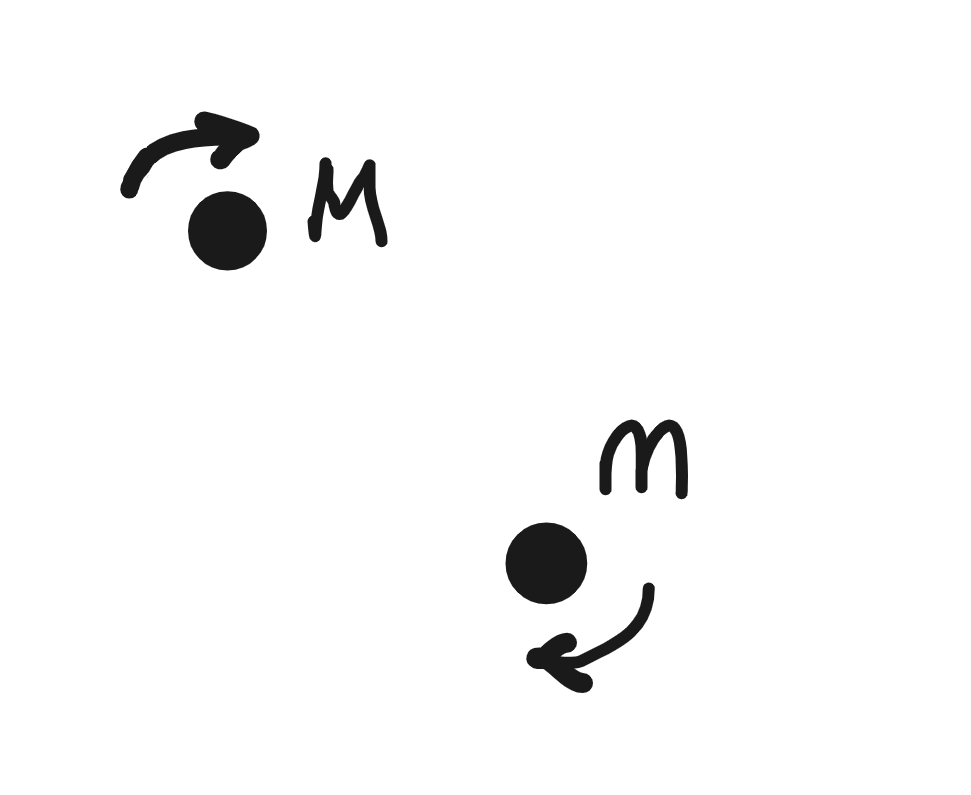
\includegraphics[scale=0.1]{autodraw.png}
\end{center}

Now, it is well known that when an electron moves it induces a magnetic moment, defined as:

$$\vec m_{moment} \equiv \frac 1 {2} e (\vec r \times vec v)$$

So, using our assumption that we simply transform electric charge to mass, we will simply replace $e$ with $m$, and assume that when a mass moves, there is a corresponding "gravitational magnetic moment":

$$\vec m_{gravitational moment} \equiv \frac 1 {2} m (\vec r \times vec v)$$

Adding in the magnetic interaction is straightforward in the low velocity limie, i.e., wehen $v << 1$. Our transformed fields will then be

$$\vec E_g' = \vec E_g$$

$$ \vec B_g' = - \vec v \times \vec E_g$$

Thus in the low velocity limit:

$$\vec B_g = - \vec v \times \vec r \frac {GM} {r^3} $$ 

The potential energy $U$ of a magnetic moment in an external field is given by:

$$U = - \vec m \cdot \vec B = \frac 1 2 m (\vec r \times \vec v)\left(\vec v \times \vec r \frac {GM} {r^3} \right) = - \frac {GMm} 2 (\vec r \times \vec v)^2$$

A similar contribution is given to the potential energy of the system when viewed from the other mass, thus doubling the above. 

Thus, with the addition of the gravitational magnetic field , the solution to Kepler's problem is modified by this additonal term:

$$ U_{\text{Einstein}} = \frac m 2 (\frac {dr} {dt})^2 - \frac {GMm} r + \frac {l^2} {2mr^2} - \frac {GMl^2}{mr^3}$$

This is the same equation that one can achieve with General Relativity. 

According to Carroll: "A similar analysis of orbits in Newtonian gravity would have produced a similar result; the general equation (5.65) would have been the same, but the effective potential (5.66) would not have had the last term. (Note that this equation is not a power series in $1/r$, it is exact.)"

The important point to note, is that in this current theory presented in this paper. This is not exact, but is only the first order approximation. Further mathematical sophistication should lead to range of tests that could be performed to see which is the true theory of nature.


\newpage
\subsection{Bending of light around a mass}
This section concerns the two classical test of General Relativity concerning the bending of light around a massive object and the blue-shift of light as it falls down towards a massive object.

Main Postulate / Hypothesis: Empty space is filled with a randomly-fluctuating zero-point energy and a massive object absorbs some of this energy, thereby preventing collapse of the mass. I therefore postulate that a massive object induces a “field” (or maybe a momentum-flow is a better way to say it? sink?) in the surrounding space and when a photon travels through this “field,” the momentum of the photon is shifted in an additive and linear manner – in accordance with the following equation: 

$$\Delta \vec p = \int_{path} \vec P ~ dl ~~~~~~~~~~~ (30)$$

where we integrate along the path of the photon and $\vec P$ is defined as

$$\vec P = - \hat r \frac {Gm\hbar}{r^2} ~~~~~~~~~~~ (31)$$

We imagine a photon that emanates from a distant source, passes close by a massive object, then continues beyond the object to an observer. The closest point while passing, i.e., the impact parameter, is at a distance of $b$ from the center of the object. For ease of calculation, we will say that both the point of emanation and the observer are infinitely far from the massive object.

\begin{center}
	\includegraphics[scale=0.4]{light-bending.png}
\end{center}


We assume that to a first-order approximation the trajectory of the photon is a straight line. To calculate its change in momentum, we integrate along the straight-line path of the photon:

$$\Delta \vec p = \int_{path} \vec P ~ dl = \int_{-\infty}^{\infty} - \frac {Gm\hbar}{r^3} \vec r ~ wdz $$

We divide the problem into two parts: the momentum change in the direction parallel to the direction of travel of the photon and the momentum change perpendicular to the direction of travel. In calculating the momentum change in the direction parallel to the direction of travel, we note that as the photon approaches and then recedes from the massive object, the change in momentum cancels out to leave zero net change in the parallel direction. We can easily calculate the change in momentum in the direction perpendicular to the direction of travel:

$$\Delta p_y = \int_{-\infty}^{\infty}  \frac {Gm\hbar}{(z^2 + b^2)^{3/2}} b ~ wdz $$

This yields:

$$\Delta p_y = \hbar w \frac {2Gm} b$$

We therefore get:

$$\theta \approx \sin \theta = \frac {\Delta p_y}{p_z} = \frac {2Gm} b$$

Which yields the deflection angle:

$$\alpha = \frac {4Gm} b$$

This is the same result as in the theory of General Relativity.

\newpage
\subsection{Light falling in a gravity well}

Using the same postulate, we can calculate the blue-shift of light. As a photon falls into a gravity well, the momentum and hence the energy of the photon are shifted. Because the energy of a photon is generally expressed as a frequency, we say that the frequency of the photon observed at infinity is changed compared to when it is observed in a gravitational field at a distance R from the center of the massive object. We use the following equation to express this change:

$$\hbar w' = \hbar w + \Delta p $$

To calculate the change in momentum, we again integrate along the path of the photon:

$$\Delta p = \int_{\infty}^R \hat r \cdot \vec P w dr= \int_{\infty}^R - \frac {Gm\hbar}{r^2} w dr = \hbar w \frac {Gm}R $$

This yields:

$$\hbar w' = \hbar w \left( 1 + \frac {Gm}R \right) $$

At lowest order approximation, this is the same as that found in General Relativity

\newpage

\section{Dirac Equation}
\subsection{Dual transform}
\newpage
\subsection{Spinor Transformation}
\newpage

\end{document}
